% ==========================================
\chapter[Diffusion Processes on Networks]{Diffusion Processes on\\Networks}
% ==========================================

% ==========================================
\section{Fundamentals of Network Diffusion}
% ==========================================

In the study of dynamical processes on complex systems, network diffusion serves as a fundamental model for phenomena ranging from random walks and heat dissipation to the spreading of information or diseases. In this framework, the \textbf{nodes} of the network represent the possible states of the system (e.g., discrete positions in space, distinct chemical reaction compounds), while the \textbf{links} represent the allowed transitions or pathways between these states.

\subsection{Markov Chains and Transition Matrices}

To mathematically describe the state of the system at any given time, we associate a value $x_i$ to the $i$-th node, which represents the probability of the system being in the $i$-th state. Consequently, the global state of the network is described by a state vector $\vec{x}$, which must be a unit $L^1$ norm probability vector satisfying two conditions:
\begin{enumerate}
    \item $x_i \ge 0$ for all $i$ (non-negativity of probabilities).
    \item $\sum_i x_i = 1$ (normalization).
\end{enumerate}

The discrete-time evolution of this system is modeled as a \textbf{Markov Chain}. We define $T_{ij}$ as the transition matrix element representing the probability of moving \textit{from} node $j$ \textit{to} node $i$. The state vector updates at each discrete time step according to the linear relation:
\[
    x_i(t+1) = \sum_{j} T_{ij} x_j(t)
\]
This equation states that the probability of finding the system at node $i$ at time $t+1$ is exactly the sum of the probabilities entering node $i$ from all possible nodes $j$ at the previous time step $t$.

Because the system must go \textit{somewhere} (including possibly staying at the same node), the probabilities of moving to any possible node $i$ from a given state $j$ must sum to unity:
\[
    \sum_{i} T_{ij} = 1
\]
This property means the transition matrix $T$ is \textit{column-stochastic}. A direct consequence of this column normalization is the strict conservation of total probability over time:
\[
    \sum_{i} x_i(t+1) = \sum_{i} \sum_{j} T_{ij} x_j(t) = \sum_{j} \left( \sum_{i} T_{ij} \right) x_j(t) = \sum_{j} 1 \cdot x_j(t) = 1
\]

\paragraph{Deriving the Transition Matrix from the Topology.}
In network science, the allowed transitions are dictated by the adjacency matrix $A$. To obtain the transition matrix $T$ from $A$, we must rescale the columns of $A$ by the total number of outgoing connections of each node. Let $K_j^{OUT} = \sum_i A_{ij}$ be the outgoing degree of node $j$. The elements of $T$ are given by:
\[
    T_{ij} = \frac{A_{ij}}{K_j^{OUT}}
\]
In matrix notation, we introduce a diagonal degree matrix $D$ where the diagonal elements are $D_{ij} = \delta_{ij} K_i^{OUT}$. The transition matrix is then elegantly written as:
\[
    T = A \cdot D^{-1}
\]

\textit{Important properties to note:}
\begin{itemize}
    \item Even if the underlying network is perfectly undirected (meaning the initial adjacency matrix $A$ is symmetric), the resulting transition matrix $T$ is generally \textbf{not symmetric} ($T_{ij} \neq T_{ji}$) unless the network is regular (i.e., all nodes share the exact same degree).
    \item Multiplying by $D^{-1}$ from the \textit{right} ($A \cdot D^{-1}$) normalizes the columns, which tracks forward probability flow. Conversely, if we were to multiply by $D^{-1}$ from the \textit{left} ($D^{-1} \cdot A$), we would normalize $T$ by rows instead of columns. By multiplying a probability vector $\vec{x}(t)$ by this row-normalized matrix from the left, we can effectively \textbf{backpropagate diffusion in time}, a technique conceptually related to solving the backward Kolmogorov equation to identify the origin of a diffusion process.
\end{itemize}

\subsection{The Master Equation and the Diffusive Laplacian}

While the Markov chain formalism describes discrete time steps, physical systems often evolve continuously. We can transition to a continuous-time formulation by defining a fundamental time step $\Delta t = 1$  and analyzing the rate of change of the probability vector:
\[
    \frac{\vec{x}(t + \Delta t) - \vec{x}(t)}{\Delta t} = (T - I) \cdot \vec{x}(t) = -(I - T) \cdot \vec{x}(t)
\]
Taking the continuous limit yields the \textbf{Master Equation} of the diffusion process:
\[
    \dot{\vec{x}}(t) = -(I - T) \cdot \vec{x}(t) = -L_T \cdot \vec{x}(t)
\]
Here, we have introduced $L_T = (I - T)$, which acts as the \textbf{``diffusion'' Laplace operator} on the network.

We can express $L_T$ explicitly in terms of the adjacency and degree matrices. By substituting $T = A \cdot D^{-1}$, we get:
\[
    L_T = I - A \cdot D^{-1} = (D - A) \cdot D^{-1}
\]
It is crucial to distinguish this operator from the standard combinatorial Laplacian $L = (D - A)$. The diffusive Laplacian $L_T = L \cdot D^{-1}$ is the \textit{random walk normalized Laplacian}. Because of the $D^{-1}$ term, it specifically governs conservative flow and probability diffusion on the graph geometry, ensuring that the total ``mass'' of the system remains invariant under the continuous time derivative ($\sum_i \dot{x}_i = 0$).

% ==========================================
\section{Stationary States and Spectral Dynamics}
% ==========================================

By viewing network diffusion as a Markov chain, we can leverage the powerful tools of linear algebra and spectral graph theory to understand the long-term behavior of the system.

\subsection{The Eigenvalue Problem}

The state of the system after $N$ discrete time steps is obtained by applying the transition matrix $T$ exactly $N$ times to the initial state vector $\vec{x}(t_0)$. Mathematically, this corresponds to a matrix multiplication power:
\[
    \vec{x}(t_N) = T^N \vec{x}(t_0)
\]


As $N \to \infty$, the system generally approaches a \textbf{stationary state} $\vec{x}_S$. A stationary state is defined as a state vector that remains unchanged by the evolution operator $T$:
\[
    \vec{x}_S = T \vec{x}_S
\]

In the continuous-time framework (the master equation), this stationary state corresponds to a state of dynamic equilibrium where the time derivative vanishes ($\dot{\vec{x}} = 0$).

The search for the stationary state is naturally formulated as an \textbf{eigenvalue problem}:
\[
    T \cdot \vec{x} = \lambda \cdot \vec{x} \quad \text{with} \quad \lambda = 1
\]


We are guaranteed that an eigenvalue of $\lambda = 1$ always exists for a column-stochastic transition matrix. This becomes evident when we look at the \textit{left} eigenvectors. Let $\vec{1} = (1, 1, \dots, 1)$ be the all-ones vector. Because the columns of $T$ sum to 1 ($\sum_i T_{ij} = 1$), multiplying $T$ from the left by $\vec{1}$ returns $\vec{1}$:
\[
    \vec{1} T = \vec{1}
\]

Because $T$ is generally asymmetric, its left and right eigenvectors are different. However, a fundamental property of matrices is that the left and right eigenvalue spectra are identical, ensuring that the right eigenvalue $\lambda = 1$ (and its corresponding stationary state eigenvector) also exists.

\subsection{Stationary States in Symmetric Networks}

If the original adjacency matrix $A$ of the network is symmetric ($A_{ij} = A_{ji}$), an exact analytical solution for the stationary state can be easily demonstrated. In such networks, the stationary state vector $\vec{x}_S$ has components that are strictly proportional to the node degree $k$:
\[
    \vec{x}_S \propto \vec{k}
\]


\textbf{Proof:} We know that the node degree is $k_j = \sum_i A_{ij}$, and the transition matrix elements are defined as $T_{ij} = \frac{A_{ij}}{k_j}$. We want to test if the degree vector $\vec{k}$ satisfies the eigenvalue equation $T\vec{k} = \vec{k}$. Evaluating the $i$-th component of $T\vec{k}$ gives:
\[
    (T\vec{k})_i = \sum_{j} T_{ij} k_j = \sum_{j} \frac{A_{ij}}{k_j} k_j = \sum_{j} A_{ij}
\]

Because the matrix $A$ is symmetric, summing over the columns $j$ of row $i$ is identical to summing over the rows $i$ of column $j$. Therefore, $\sum_j A_{ij} = \sum_j A_{ji} = k_i$. Thus, $T\vec{k} = \vec{k}$, proving that the degree vector is indeed the eigenvector corresponding to $\lambda = 1$.

\subsection{Transient Dynamics and Numerical Solutions}

To understand how the system approaches this stationary state, we can decompose the initial state $\vec{x}(0)$ into a linear combination of the eigenvectors $\vec{x}^{(\lambda_i)}$ of the transition matrix:
\[
    \vec{x}(0) = \sum_i c_i \cdot \vec{x}^{(\lambda_i)}
\]

Evolving this state forward in time by applying $T^N$ yields:
\[
    \vec{x}(N\tau) = T^N \vec{x}(0) = \sum_i c_i \cdot \lambda_i^N \cdot \vec{x}^{(\lambda_i)}
\]

We can factor out the dominant (maximum) eigenvalue $\lambda_{MAX}^N$:
\[
    \vec{x}(N\tau) = \lambda_{MAX}^N \sum_i c_i \cdot \left( \frac{\lambda_i}{\lambda_{MAX}} \right)^N \cdot \vec{x}^{(\lambda_i)}
\]

Because $\lambda_{MAX}$ is the largest eigenvalue, for all other eigenvectors $\lambda_i < \lambda_{MAX}$, the fraction $\frac{\lambda_i}{\lambda_{MAX}}$ is strictly less than 1. Consequently, as $N \to \infty$, the term $\left( \frac{\lambda_i}{\lambda_{MAX}} \right)^N \to 0$. These non-dominant eigenvectors represent \textbf{transient states} that decay geometrically in discrete time (or exponentially in the continuous limit). Eventually, only the component associated with $\lambda_{MAX}$ survives, which is the stationary state.

\paragraph{Numerical Solutions (Power Iteration).}
For very large complex systems, solving the eigenvalue problem analytically becomes computationally unfeasible. Instead, numerical approximations are required. Based on the decay of transient states shown above, we can isolate the dominant eigenvector by repeatedly multiplying an arbitrary initial state vector $\vec{v}$ by the matrix $A$ (or $T$).
\[
    \lim_{N \to \infty} A^N \cdot \frac{\vec{v}}{|\vec{v}|} = \vec{x}^{(\lambda_{MAX})}
\]

Similarly, the dominant eigenvalue itself can be numerically extracted by taking the ratio of successive iterations:
\[
    \lim_{N \to \infty} \frac{A^{N+1} \cdot \vec{v}}{A^N \cdot \vec{v}} = \lambda_{MAX}
\]


\paragraph{The Rayleigh Principle.}
Another profound way to frame the eigenvalue problem is through functional optimization using the \textbf{Rayleigh principle}. The dominant eigenvalue can be found by maximizing the Rayleigh functional:
\[
    \lambda_{MAX} = \max \left( \frac{\vec{x}^T \cdot A \cdot \vec{x}}{\vec{x}^T \cdot \vec{x}} \right)
\]

The vector $\vec{x}$ that maximizes this quotient is precisely the dominant eigenvector $\vec{x}_{MAX}$. The remaining eigenvectors can be calculated analogously via constrained maximization, restricting the search space to the subspace orthogonal to the previously obtained eigenvectors ($\vec{x} \perp \vec{x}_\lambda$). Conversely, function minimization of the Rayleigh quotient will yield the smallest eigenvalue.

% ==========================================
\section{The Perron-Frobenius Theorem}
% ==========================================

When dealing with the spectral dynamics of diffusion, two fundamental mathematical questions naturally arise:
\begin{enumerate}
    \item Are we always guaranteed to find a maximal eigenvalue that is strictly unique (which would ensure a single, well-defined stationary state)?
    \item What physical properties does the eigenvector associated with this maximal eigenvalue possess?
\end{enumerate}

These questions are elegantly answered by the \textbf{Perron-Frobenius (P-F) Theorem}, a cornerstone of matrix algebra. The theorem is particularly powerful because it applies specifically to \textbf{non-negative matrices}—a class that perfectly encapsulates network graphs with positive link weights and transition probability matrices (Markov chains).

\subsection{Statement of the Theorem}

The Perron-Frobenius theorem establishes the conditions under which a network will converge to a single, physically meaningful steady state.

\textbf{Theorem Statement:} Let $A$ be a real, non-negative matrix that is both \textit{irreducible} and \textit{primitive}. Under these conditions:
\begin{enumerate}
    \item $A$ possesses a dominant, real eigenvalue $\lambda_{MAX}$ that is strictly greater in absolute value than all other complex eigenvalues of the matrix: $\lambda_{MAX} > |\lambda|$.
    \item The corresponding eigenvector $\vec{x}_{MAX}$ has strictly \textbf{real and positive values} ($x_i > 0 \, \forall i$). This holds true even if the matrix $A$ is completely asymmetric.
    \item The eigenvalue $\lambda_{MAX}$ has an algebraic multiplicity of exactly 1, meaning the maximal eigenvalue is unique.
\end{enumerate}

In the context of network diffusion and Markov chains (where $A$ becomes the transition matrix $T$), the dominant eigenvalue is $\lambda_{MAX} = 1$. The P-F theorem guarantees that the resulting stationary distribution vector $\vec{x}_S$ will not contain any negative or complex probabilities, nor will it assign a zero probability to any node, provided the topological conditions are met.

\subsection{Topological Conditions: Irreducibility and Primitivity}

The theorem relies on two strict topological conditions: irreducibility and primitivity. Understanding when networks violate these conditions helps us understand pathological diffusion behaviors.

\subsubsection{1. Irreducibility (Strong Connectivity)}

A matrix is \textbf{irreducible} if and only if the underlying directed graph is \textit{strongly connected}. This means that for every pair of nodes $i$ and $j$, there exists at least one directed path from $i$ to $j$, and vice versa.

If a network is \textit{reducible}, it contains separated subsystems or ``absorbing states.'' In linear algebra terms, a reducible matrix can be transformed via a basis change (using an invertible matrix $B$) into an upper block-triangular form:
\[
    \exists B \quad \text{such that} \quad B^{-1} A B = \begin{pmatrix} A_{11} & A_{12} \\ 0 & A_{22} \end{pmatrix}
\]
Physically, this represents a network where probability mass or traffic can flow from the nodes in block $A_{11}$ to the nodes in block $A_{22}$ (via $A_{12}$), but can never return because the bottom-left block is strictly zero. Consequently, $A_{22}$ acts as an absorbing basin or sink. In such cases, the network will completely drain into the absorbing states, and the corresponding stationary eigenvector will feature zero values for all nodes in the transient block $A_{11}$, violating the positivity condition of the P-F theorem.

\subsubsection{2. Primitivity (Aperiodicity)}

While irreducibility ensures there are no dead ends, \textbf{primitivity} ensures there are no infinite oscillatory loops. A primitive matrix is one that is non-negative, irreducible, and \textit{aperiodic}.

A matrix fails to be primitive (it is \textit{imprimitive}) if it represents a perfectly multipartite graph—groups of nodes that only connect to other distinct groups in a strict cycle. Imprimitivity implies that the dominant eigenvalue is not strictly unique in magnitude; there are multiple eigenvalues on the spectral circle ($\#(\lambda_{MAX}) > 1$ in terms of absolute value).

A classic example of an imprimitive matrix takes a cyclic block form:
\[
    A_{cyclic} = \begin{pmatrix} 0 & A_1 & 0 \\ 0 & 0 & A_2 \\ A_3 & 0 & 0 \end{pmatrix}
\]
In a diffusion process on this topology, the system never settles into a stationary distribution. Instead, the probability mass shifts entirely from block 1, to block 2, to block 3, and back to block 1, infinitely. These ``cyclic'' solutions mean the state values ``switch'' forever between components, violating the convergence property. Additionally, an imprimitive matrix does not satisfy $A^K = A$ for any macroscopic power due to its periodicity.

\paragraph{Conclusion for Transition Matrices.}
For a Markov chain transition matrix to behave nicely, we must ensure it is both irreducible (no absorbing sinks or isolated subsystems) and primitive (no cyclic communicating blocks). When these two conditions are satisfied, the Perron-Frobenius theorem ensures the existence of a \textbf{unique stationary distribution} strictly greater than zero across the entire network.

% ==========================================
\section{Eigenvector Centrality Variations: PageRank}
% ==========================================

A highly impactful variation of eigenvalue centrality is the \textbf{PageRank} algorithm, famously developed by Brin and Page in 1998 to rank website relevance for the Google search engine. In essence, the PageRank score of a website is mathematically defined as the stationary state of a diffusion process on the World Wide Web, which is modeled as a massive directed network of hyperlinks.

\subsection{The Random Surfer and the Damping Factor}

In a directed network, relying purely on standard eigenvector centrality or simple diffusion is problematic. The hyperlink network of the web is not guaranteed to be strongly connected; it contains many isolated components, ``sink'' nodes with no outgoing links, and cyclic traps. To solve this, PageRank introduces a ``smart'' additional term.

The conceptual model is that of a ``random surfer.'' The surfer navigates the web by randomly clicking on available outgoing links. The PageRank $PR(A)$ of a node (page) $A$ depends on the PageRank of the $k$ nodes pointing to it, scaled inversely by the number of outgoing links $C(k)$ from each of those $k$ nodes. In other words:
\begin{itemize}
    \item The higher the PageRank of the webpages pointing at you, the better.
    \item However, if a highly-ranked webpage points to many different pages, its conveyed importance is linearly diluted among all its targets.
\end{itemize}

To prevent the surfer from getting stuck in absorbing states or disconnected components, we introduce a \textbf{damping factor}, $d$ (typically set to $0.85$). With probability $1-d$, the surfer abandons the current link structure and ``teleports'' to a completely random page anywhere on the web.

The formula for the PageRank score of node $A$ is written as:
\[
    PR(A) = (1 - d) + d \left( \sum_{k} \frac{PR(k)}{C(k)} \right)
\]

In vector and matrix notation, letting $\vec{x}$ be the vector of PageRank scores (where $\sum_i x_i = 1$) and $T$ be the column-normalized transition matrix derived from the adjacency matrix, we can express this as:
\[
    \vec{x} = d \cdot T\vec{x} + (1 - d)\vec{1}
\]

\paragraph{Ensuring Perron-Frobenius Conditions.}
Because we must ensure the network is strongly connected to find a valid stationary state, the algorithm employs a clever mathematical trick. We define a completely connected matrix $C$, where every single element is $1$. The ``teleportation'' term can be represented using this matrix. Since $\vec{x}$ is a probability vector ($\sum_i x_i = 1$), multiplying it by $\frac{C}{N}$ returns the all-ones vector scaled by $\frac{1}{N}$:
\[
    \frac{C}{N} \cdot \vec{x} = \vec{1} \cdot \frac{1}{N}
\]
*(Note: The slides use $(1-d)\vec{1}$ loosely to represent the uniform redistribution of probability, which mathematically acts as $(1-d)\frac{C}{N}\vec{x}$ in the closed linear system).*

By combining the topological transitions and the random jumps, the system evolves according to a new, effective transition matrix:
\[
    \vec{x} = \left( d \cdot T + (1 - d)\frac{C}{N} \right) \vec{x}
\]
The addition of the uniform connectivity matrix $C$ guarantees that every node is at least weakly connected to every other node. Therefore, the new effective transition matrix is strictly positive, satisfying both the \textbf{irreducibility} and \textbf{primitivity} conditions. By the Perron-Frobenius theorem, this guarantees a unique stationary state solution where all PageRank scores are strictly positive, corresponding to the maximum eigenvalue.

\subsection{Analytical and Numerical Formulation}

To find the stationary state $\vec{x}$, we can attempt an analytical solution. Starting from $\vec{x} = d \cdot T\vec{x} + (1 - d)\vec{1}$, we can rearrange the terms:
\[
    (I - d \cdot T)\vec{x} = (1 - d)\vec{1}
\]
By inverting the matrix $(I - d \cdot T)$, we obtain the exact analytical solution:
\[
    \vec{x} = (1 - d)(I - d \cdot T)^{-1}\vec{1}
\]
The positive values of the resulting eigenvector $\vec{x}$ (guaranteed by the P-F theorem) are the definitive webpage ranking scores.

\paragraph{The Need for Numerical Iteration.}
While mathematically elegant, calculating the exact analytical solution via matrix inversion is computationally unfeasible in practice. Matrix inversion has a complexity of $\mathcal{O}(N^3)$, and the network of the World Wide Web consists of billions of websites.

The standard solution is to \textbf{numerically iterate} the diffusion process. We define the iterative step using the effective transition matrix $P = d \cdot T + (1 - d)\frac{C}{N}$:
\[
    \vec{x}(t+1) = P \cdot \vec{x}(t)
\]
Starting from an initial random guess $\vec{x}(0)$, we apply $P$ repeatedly. After a sufficient number of steps $N \gg 1$, the transient states decay, and the vector gets closer to the convergence of the stationary state $\vec{x}_S$:
\[
    \vec{x}_S = \lim_{N \to \infty} P^N \vec{x}(0)
\]
The speed at which this numerical approach converges to the stationary state depends heavily on the spectral gap—specifically, the relationship between the dominant eigenvalue (which is 1) and the second largest eigenvalue of the matrix $P$.

% ==========================================
\section{Random Walk Betweenness}
% ==========================================

Standard Betweenness Centrality (BC) is built on a very strong and somewhat idealized assumption: that information, traffic, or physical flow in a network always travels exclusively along the absolute shortest paths. While mathematically elegant, this assumption is often violated in real-world scenarios. In systems like vehicular traffic, the internet, or social gossip, agents may lack perfect global knowledge of the network or intentionally choose slightly longer, alternative routes to avoid congestion.

To capture a more realistic model of flow, we introduce \textbf{Random Walk Betweenness (RWB)}. This centrality measure evaluates the importance of a node based on the expected number of times it is traversed by a random walk. Because a random walker explores the network probabilistically, RWB considers \textit{all} possible paths, not just the shortest ones.

\subsection{Pathological Cases of Standard Betweenness}

The limitations of shortest-path BC become starkly apparent in certain ``pathological'' topological configurations, where near-optimal alternative roads are completely ignored.

\begin{figure}[ht]
    \centering
    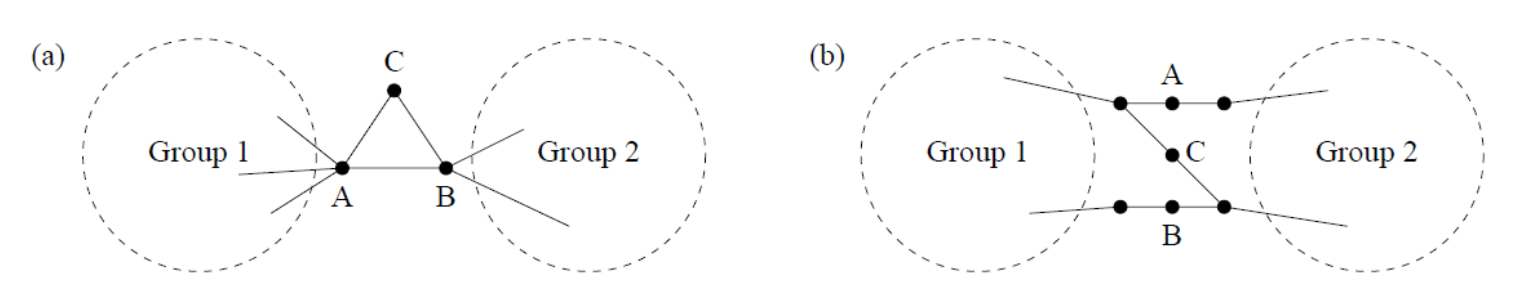
\includegraphics[width=0.9\textwidth]{img/pathological_BC.png}
    \caption{Pathological cases in Betweenness Centrality: (a) The Triangle Bridge and (b) Parallel Bridges.}
    \label{fig:pathological_bc}
\end{figure}

Consider the two configurations in the referenced figure:
\begin{itemize}
    \item \textbf{Configuration (a) - The Triangle Bridge:} Two dense communities (Group 1 and Group 2) are connected by three nodes, $A$, $B$, and $C$, arranged in a triangle. Nodes $A$ and $B$ are directly connected to the groups and to each other. Because the direct path $A \to B$ is length 1, the path $A \to C \to B$ (length 2) is strictly sub-optimal. Consequently, nodes $A$ and $B$ will accumulate massive standard BC scores, while node $C$ will have a BC of exactly zero. Yet, structurally, $C$ provides a highly relevant alternative bridge.
    \item \textbf{Configuration (b) - Parallel Bridges:} In cases of multiple parallel links between communities, BC can heavily skew towards one specific path depending on minute weight differences, entirely discounting redundant, slightly longer paths.
\end{itemize}

Random Walk Betweenness resolves this. By comparing a node's standard BC with its Random Walk BC (often using a scatterplot of the two measures or analyzing their numerical difference), one can easily identify these hidden ``alternative route'' nodes that standard algorithms miss.

\subsection{Markov Chains and Walk Probabilities}

To formalize Random Walk Betweenness, we model the diffusion process as a Markov chain. Let us define a random walk transition matrix $M$, where $M_{ij}$ represents the probability of moving \textit{from} node $j$ \textit{to} node $i$ in a single step. If the network is unweighted, this is simply the inverse of the outgoing degree:
\[
    M_{ij} = p(i|j) = \frac{A_{ij}}{k_j}
\]
By definition, the sum over all possible destinations $i$ from a given origin $j$ is normalized: $\sum_i M_{ij} = 1$.

If $M_{ij} = 0$, a direct 1-step transition from $j$ to $i$ is impossible. However, the walker could reach $i$ in 2 steps by passing through an intermediate node $k$ (i.e., $j \to k \to i$). The probability of this specific 2-step path is $M_{ik} \cdot M_{kj}$. To find the total probability of transitioning from $j$ to $i$ in exactly 2 steps across \textit{all} possible intermediate nodes, we sum these products, which is simply the matrix multiplication $M^2$:
\[
    [M^2]_{ij} = \sum_k M_{ik} \cdot M_{kj}
\]

By induction, the probability of going from $j$ to $i$ in exactly $N$ steps is proportional to the $ij$-th element of the matrix $M^N$:
\[
    P(j \to i \text{ in } N \text{ steps}) \propto [M^N]_{ij}
\]

\paragraph{Intrinsic Path Weighting.}
This formulation inherently solves the problem of weighting paths by their length. Because the transition probabilities are fractional ($M_{ij} < 1$ for nodes with degree $>1$), the elements of $M^N$ become progressively smaller as $N$ increases. Therefore, while RWB counts all possible walks, very long, meandering walks contribute exponentially less to the centrality score than short, direct paths. The walks are automatically weighted by their length.

\paragraph{Infinite Random Walks and Convergence.}
To compute the total expected number of passages through a target node $j$ when starting a random walk from a source node $s$, we must sum the probabilities over all possible time steps $r$ from $0$ to infinity:
\[
    \sum_{r=0}^{\infty} P(j | t=r) = \sum_{r=0}^{\infty} [M^r]_{js}
\]
This is a geometric series of matrices. Because the magnitude of the eigenvalues of the strictly transient parts of the random walk matrix $M$ is strictly less than 1 ($|\lambda| < 1$), this matrix geometric series converges:
\[
    \sum_{r=0}^{\infty} M^r = (I - M)^{-1}
\]
Thus, the total expected passages through $j$ from $s$ is given by the $js$-th entry of the matrix $(I - M)^{-1}$.

\textit{Note for future derivation:} If we want to consider the probability of the walker making one further movement exiting node $j$, we can multiply this result by $\frac{1}{k_j}$. This mathematical trick will become highly relevant when linking this concept to the graph Laplacian.

% ==========================================
\subsection{Absorbing States and the Laplacian Pseudoinverse}
% ==========================================

To calculate the expected number of times a random walker passes through a specific node, we evaluate the infinite sum of the transition matrix powers, $\sum_{r=0}^{\infty} M^r = (I - M)^{-1}$. This infinite geometric series is deeply connected to the network's Laplacian matrix.

By substituting the unweighted transition matrix definition $M = A D^{-1}$ (where $A$ is the adjacency matrix and $D$ is the diagonal degree matrix), we can manipulate the inverse expression:
\[
    (I - M)^{-1} = (I - A D^{-1})^{-1} = \left( (D - A)D^{-1} \right)^{-1} = D(D - A)^{-1} = D L^{-1}
\]
Here, $L = D - A$ represents the standard combinatorial graph Laplacian.
If we consider an additional ``exit'' step from the target node $j$, which occurs with probability $1/k_j$, we effectively multiply the right side by $D^{-1}$. This elegantly reduces the equation exactly to the inverse Laplacian $L^{-1}$. Thus, the total number of passages through a node during an infinite random walk is fundamentally governed by the inverse of the Laplacian matrix.

\paragraph{The Singularity Problem and the Absorbing State Trick.}
A critical mathematical issue arises here: the Laplacian matrix $L$ always has at least one eigenvalue equal to zero ($\lambda_1 = 0$, corresponding to the all-ones eigenvector $\vec{1}$), meaning its determinant is zero ($|L|=0$) and the matrix is strictly non-invertible.

To bypass this singularity, we can use the \textbf{absorbing state trick}. We define our destination node $t$ as an ``absorbing state'', meaning that once the random walker reaches $t$, it can never leave. Mathematically, we force all transition probabilities out of $t$ to zero:
\[
    M_{it} = 0 \quad \forall i
\]
In matrix terms, this corresponds to deleting the $t$-th row and $t$-th column from the transition matrix (or the Laplacian), resulting in a ``reduced'' sub-matrix $M_t$ (or $L_t$). Because the zero-eigenvalue is removed along with the grounded node, this reduced matrix \textit{is} invertible. We can calculate the random walk passages through any intermediate node using this inverted reduced matrix, and simply insert zeros back for the $t$-th row and column afterward. By summing these values over all possible source-target pairs $(s, t)$, we obtain the Random Walk Betweenness for edges and nodes.

\paragraph{The Moore-Penrose Pseudoinverse.}
Alternatively, instead of grounding a specific node, we can compute the \textbf{pseudoinverse} (often denoted as $L'$ or $L^+$) using spectral decomposition. Given the eigenvalues $\lambda_i$ and the corresponding orthonormal eigenvectors $\vec{u}_i$ of the symmetric Laplacian $L$, the matrix can be projected as:
\[
    L = \sum_{i=1}^{N} \lambda_i \cdot \vec{u}_i \cdot \vec{u}_i^T
\]
Because the singularity is caused solely by the first eigenvalue $\lambda_1 = 0$, the pseudoinverse is constructed by simply skipping the first term and inverting the non-zero eigenvalues:
\[
    L' = \sum_{i=2}^{N} \frac{1}{\lambda_i} \cdot \vec{u}_i \cdot \vec{u}_i^T
\]
This pseudoinverse $L'$ allows us to handle random walk calculations symmetrically without artificially removing nodes.

% ==========================================
\subsection{Hitting Time and Commute Time Distance}
% ==========================================

The pseudoinverse provides a powerful framework for defining topological distances based on random walks, moving beyond simple shortest-path geodesics.

We define the \textbf{Hitting Time} $H_{ij}$ as the expected (average) number of random jumps required for a walker to travel from node $i$ to node $j$. Note that in general networks, hitting time is asymmetric ($H_{ij} \neq H_{ji}$) because it might be ``downhill'' (easier) to reach a hub from a leaf than vice versa.

To create a proper, symmetric metric, we define the \textbf{Commute Time Distance (CTD)} $C_{ij}$, which is the expected number of jumps to walk from $i$ to $j$ \textit{and back} to $i$:
\[
    C_{ij} = H_{ij} + H_{ji}
\]

Using the Laplacian pseudoinverse $L'$, the Commute Time Distance can be calculated analytically. Let $\vec{e}_i = [0, \dots, 1, \dots, 0]^T$ be the standard basis vector for node $i$. The CTD is proportional to the quadratic form of the pseudoinverse:
\[
    C_{ij} = \left( \sum_{k} k_k \right) \cdot (\vec{e}_i - \vec{e}_j)^T L' (\vec{e}_i - \vec{e}_j)
\]
where $\sum_k k_k$ is the total volume of the network degrees.

\paragraph{CTD as a Euclidean Embedding.}
A profound consequence of this mathematical structure is that the Commute Time Distance acts as a pure squared Euclidean distance in a transformed space. By decomposing the pseudoinverse, we can map every node $i$ to a coordinate vector $\vec{\Psi}_i$ in an $(N-1)$-dimensional Euclidean space:
\[
    \vec{\Psi}_i = \sqrt{\sum_{k} k_k} \cdot (\Lambda')^{-1/2} U^T \vec{e}_i
\]
where $\Lambda'$ is the diagonal matrix of inverted non-zero eigenvalues and $U$ contains the eigenvectors.

In this new embedding space, the Commute Time Distance between any two nodes is exactly their squared Euclidean distance:
\[
    C_{ij} = || \vec{\Psi}_i - \vec{\Psi}_j ||^2
\]
Nodes that are deeply connected by many redundant short paths (e.g., within the same dense community) will be clustered very close together in this $\vec{\Psi}$ space, whereas nodes separated by bottlenecks will be pushed far apart.

\paragraph{Physical Analogy.}
The mathematical framework of Random Walk Betweenness is profoundly connected to the laws of electromagnetism. In fact, calculating the expected number of random walk passages through a node is mathematically equivalent to calculating the current flowing through a component in an electrical circuit, where edges act as resistors. The full derivation of this equivalence, known as \textbf{Current Flow Centrality}, is provided in Appendix~\ref{app:electrical_analogy}.